% !TeX root = ../../libro.tex
% !TeX encoding = utf8


\begin{teorema} (de ``alisamiento de asas'')
	Sea S una variedad diferenciable, entonces:
	\begin{enumerate}
		\item Un embebimiento $\mathbb{R}^2 \rightarrow S$ puede isotoparse a un embebimiento diferenciable en un entorno compacto del origen. Además, la isotopía coincide con la identidad fuera de un entorno compacto que contiene al anterior.
		\item Un embebimiento $D^1\times\mathbb{R} \rightarrow S$ que es diferenciable entorno a $\partial D^1\times\mathbb{R}$ puede isotoparse a un embebimiento diferenciable entorno a $D^1\times 0$. Dicha isotopía coincide con la identidad fuera de un entorno compacto de $(D^1 \times 0) \cup (\partial D^1\times\mathbb{R})$.
		\item Un embebimiento $D^2 \rightarrow S$ que es diferenciable entorno a $\partial D^2$ puede isotoparse a un embebimiento diferenciable en todo $D^2$. La isotopía coincide con la identidad en un entorno de $\partial D^2$.
	\end{enumerate}
\end{teorema}

\begin{proof}
	Voy a proceder a la demostración de cada uno de los apartados: \\
	\begin{enumerate}
		\item La idea de la demostración es arrastrar la estructura diferenciable de $S$ ($E_S$) a una estructura diferenciable sobre el Toro ($T_S$) , y aprovechar que en tales condiciones existe un difeomorfismo de $T_S$ al Toro con la estructura diferenciable estándar (por el \textbf{Hecho 4}), que nos permitirá construir la isotopía deseada.\\
			\\ Vamos a utilizar el ``truco del toro'' de Kirby, para ello veremos el toro $T$ como el espacio de órbitas $\mathbb{R}^2/\mathbb{Z}^2$ con su estructura topológica y diferenciable estándar, tomando el $0$ como imagen del $0\in \mathbb{R}^2$. Eliminamos un punto del toro distinto del $0$, y a esta nueva variedad la llamamos $T'$. \\
			\\ Consideremos una inmersión $q: T' \rightarrow \mathbb{R}^2$ diferenciable que fija el $0$. Dicha inmersión se puede construir partiendo del embebimiento del toro punteado $T'$ en un disco con dos ``1-asas'' en $\mathbb{R}^3$ y seguidamente ``aplanando'' la figura, es decir, llevar diferenciablemente el disco con asas a $\mathbb{R}^2$. Las asas se embeben por separado ya que como se observa, se solapan en $\mathbb{R}^2$.\\
			
			\begin{figure}[h]
  				\centering
  				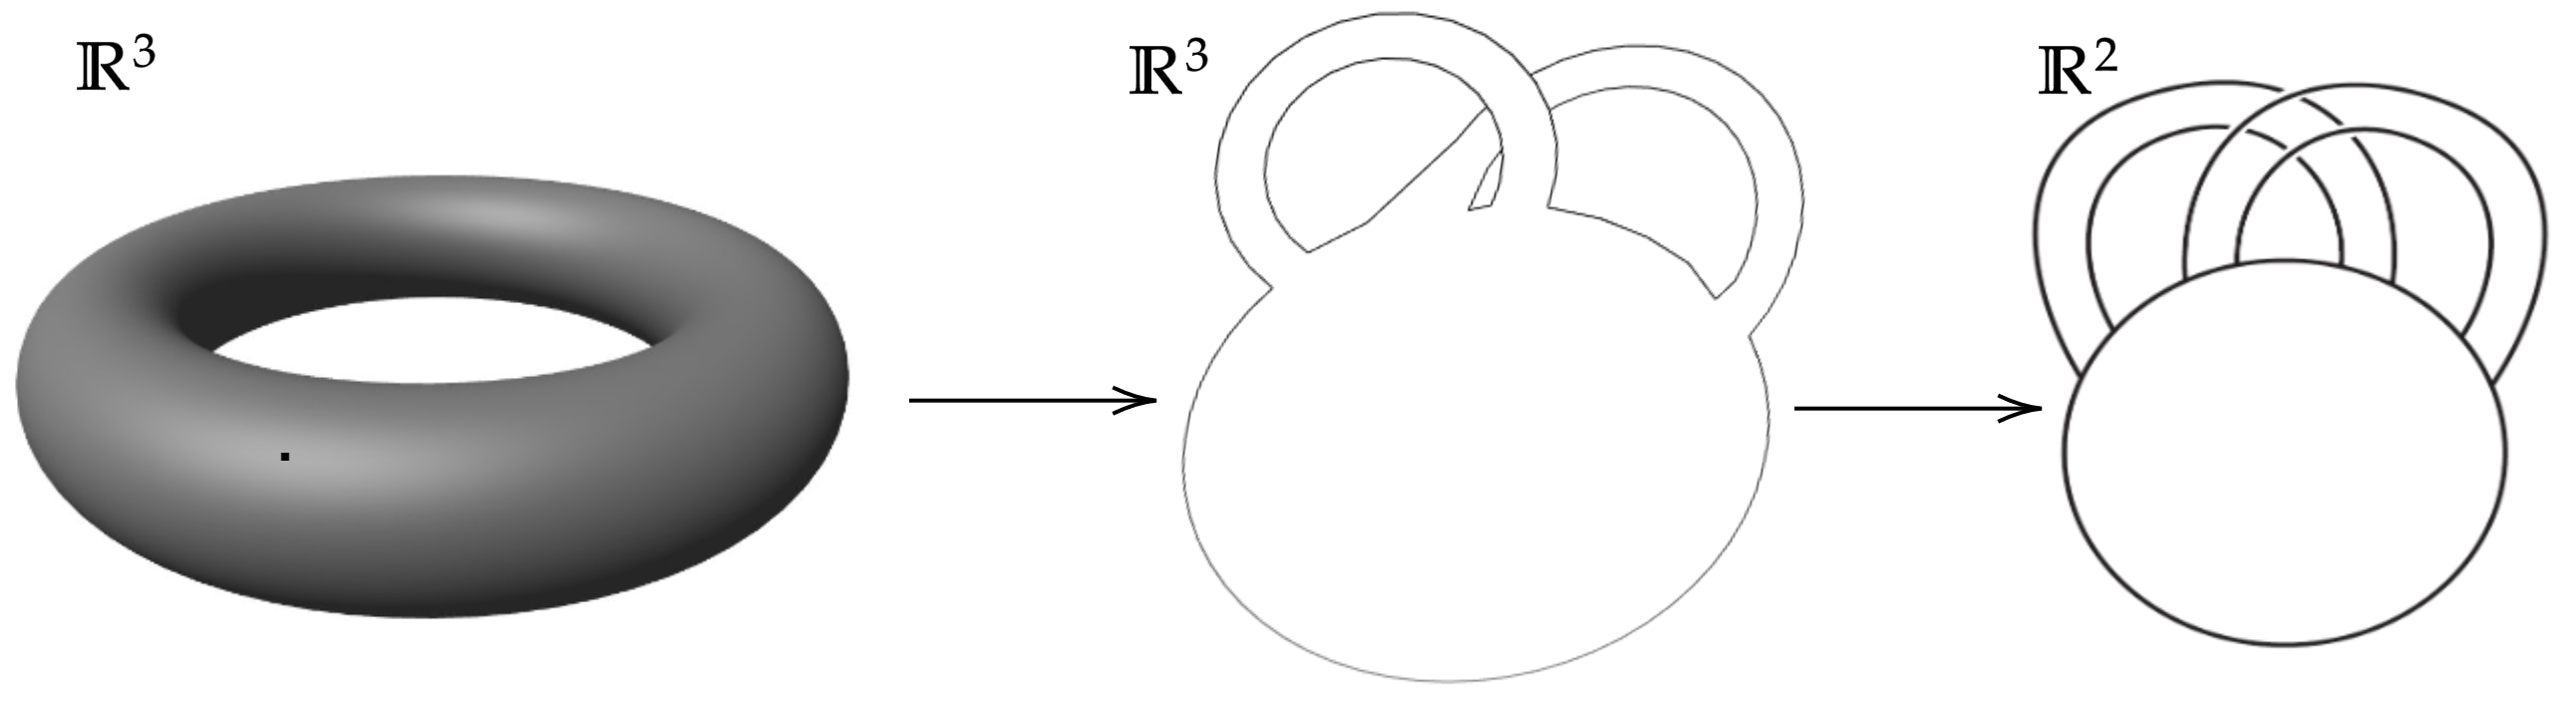
\includegraphics[width=0.8\textwidth]{toro_punteado}
  				\label{fig:toro_punteado}
			\end{figure}
			
			Sea $h:\mathbb{R}^2 \rightarrow S$ el embebimiento del enunciado, por el cual, haciendo ``pull-back'', $S$ induce una estructura diferenciable en $\mathbb{R}^2$, que denotaremos $E_1$. Por el mismo razonamiento pero para la inmersión $q$, $\mathbb{R}^2$ con la estructura $E_1$ induce una estructura diferenciable en $T'$ que llamaremos $E_2$.\\
			\\ Sabemos por el \textbf{Hecho 3} que existe un conjunto compacto en $T'_{E_2}$ cuyo complemento es difeomorfo a $S^1\times \mathbb{R}$ con su estructura diferenciable estándar, equivalentemente es difeomorfo a $D^2 - {(0,0)}$ como abierto de $\mathbb{R}^2$ con su estructura diferenciable estándar. Si vemos el disco punteado como un subconjunto del plano complejo $\mathbb{C}$, el $0$ se puede añadir de forma natural puesto que la estructura diferenciable usada hasta el momento es la usual en el cilindro (que induce la usual en $D^2$, en el plano complejo y en la esfera de Riemann). Esto nos permite extender la estructura diferenciable $E_2$ de $T'$ a $T$, la cual seguiremos llamando $E_2$.\\
			\\ Por el \textbf{Hecho 4} sabemos que toda estructura diferenciable del toro ($T \equiv S^1\times S^1$) es difeomorfa a la estándar. Por tanto, existe un difeomorfismo $g: T_{E_2} \rightarrow T$. Para poder utilizar el Teorema de Levantamiento de aplicaciones de la teoría de recubridores, necesitamos normalizar dicha función $g$:
						
			\begin{itemize}
				\item Aplicando rotaciones en el toro $T$ (lo vemos como $S^1\times S^1$) podemos hacer que $g$ lleve el $0$ en el $0$.
				\item Necesitamos que el homomorfismo $g_*$ sea la identidad a nivel de grupos fundamentales para que el difeomorfismo $g$ pueda ser levantado a un difeomorfismo $\widehat{g} : \mathbb{R}^2_{E_1} \rightarrow \mathbb{R}^2$ fijando el origen. Para ello basta con componer $g$ con el automorfismo lineal $L \in GL_2(\mathbb{Z})$ apropiado, es decir, aquel tal que al componerlo con $g_*$ queden fijos los dos generadores del grupo fundamental del toro topológico. La nueva $g$ sigue llevando el $0$ en el $0$ y $g_*$ es la identidad.\\
			\end{itemize}
			
			\begin{figure}[h]
  				\centering
  				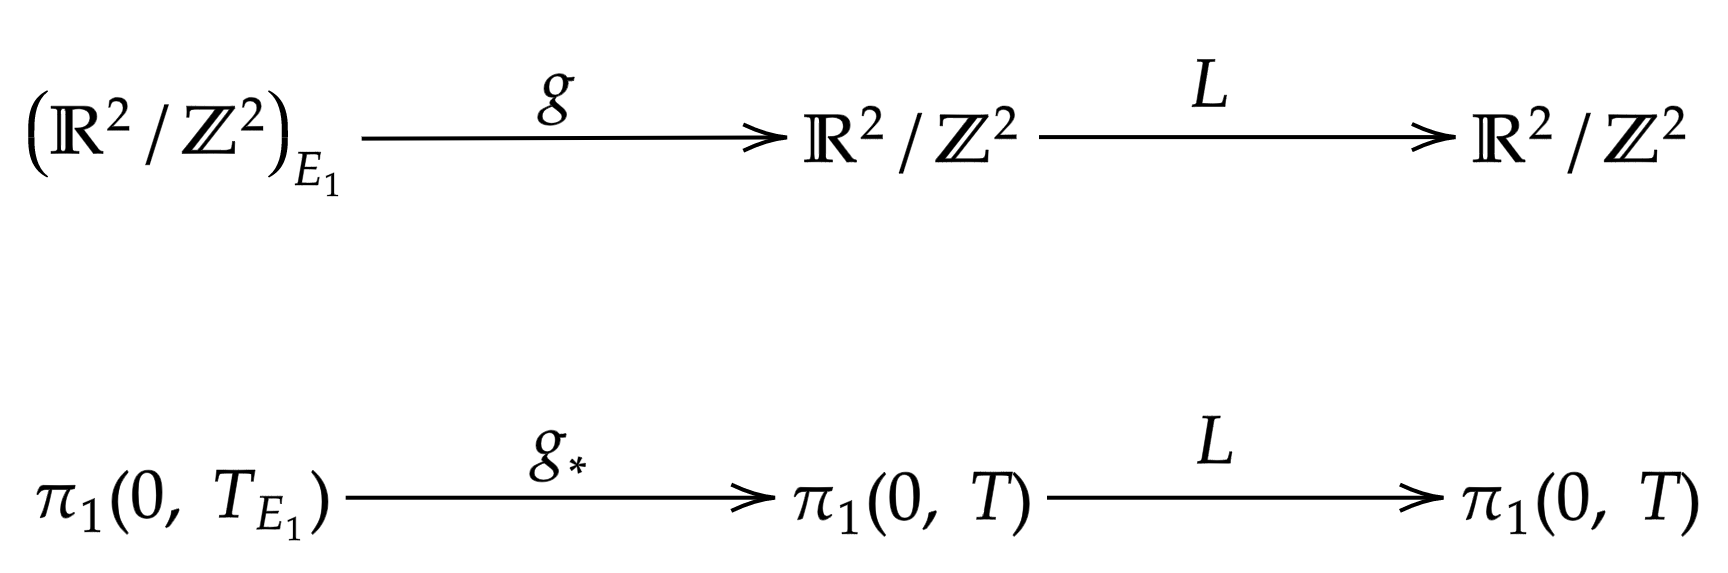
\includegraphics[width=0.5\textwidth]{grupos_fundamentales}
  				\label{fig:fundamental}
			\end{figure}
			 
			De esta forma construimos un difeomorfismo $\widehat{g}:\mathbb{R}^2_{E_1} \rightarrow \mathbb{R}^2$ como el levantamiento de $g$ fijando el origen, que de forma natural es doblemente periódico.\\
			
			\begin{figure}[h]
  				\centering
  				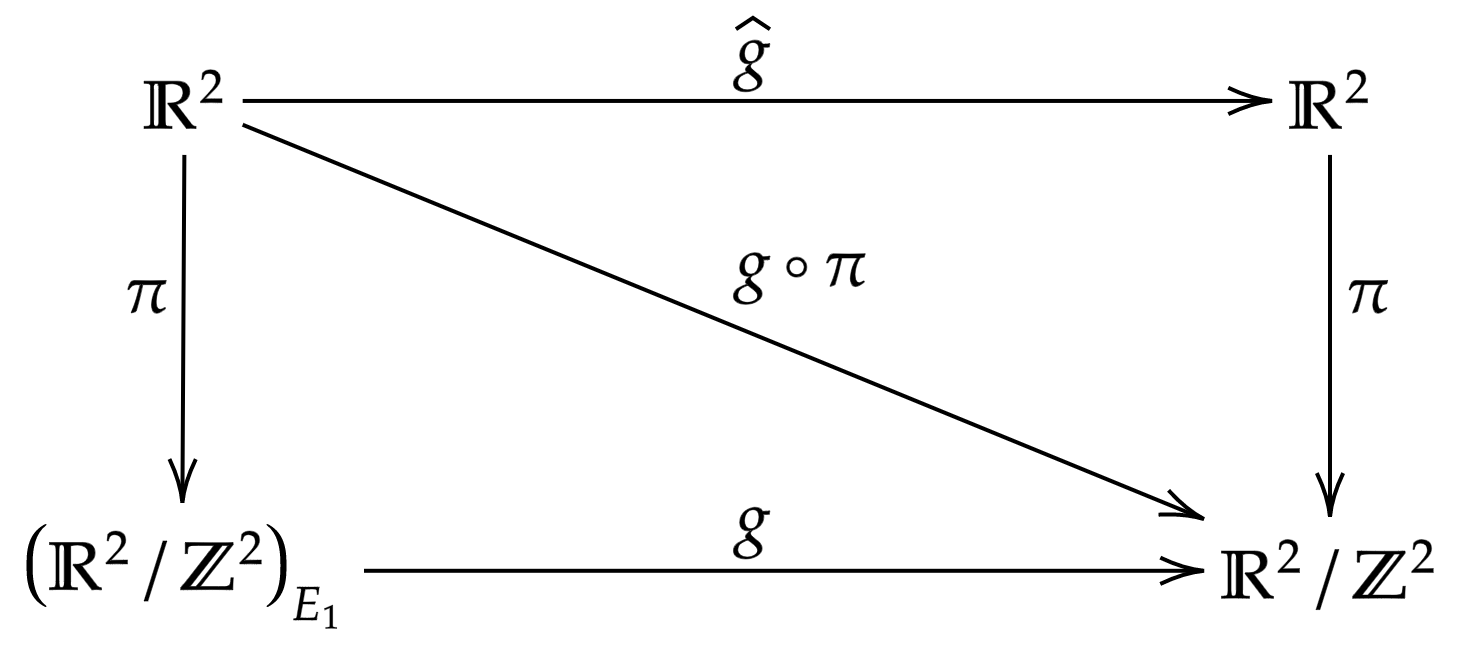
\includegraphics[width=0.5\textwidth]{levantamiento}
  				\label{fig:levantamiento}
			\end{figure}
			
			Identifiquemos $\mathbb{R}^2$ con el interior del disco unidad de $\mathbb{R}^2$ mediante una reparametrización radial que es la identidad entorno al $0$, haciendo ``pull-back'' para cada disco de $\mathbb{R}^2$ para así obtener la estructura diferenciable inducida por $E_1$, que llamaremos $E$. Entonces aplicando esta identificación en el dominio y la imagen de $\widehat{g}$ obtenemos $G:D^2_{E} \rightarrow D^2$ automorfismo diferenciable, que sigue siendo $\widehat{g}$ entorno al $0$ y tiende a ser la identidad en el borde (por la periodicidad $\|\widehat{g}(x) - x\|$ está acotado para todo $x$, y por consiguiente al tender $x$ a infinito las variaciones tienden a $0$ con la reparametrización, es decir, $G(x)$ tiende a $x$). Podemos extender $G$ a un homeomorfismo $G:\mathbb{R}^2_{E} \rightarrow \mathbb{R}^2$, siendo la identidad fuera del interior del disco.\\
			\\ Por el truco de Alexander, $G$ es isotópica a la identidad. Se puede obtener la isotopía $G_t$ variando el radio del disco de origen y destino ($G_t(x) = tG(\frac{x}{t})$ para $x \in D((0,0), t)$ y es la identidad fuera), por lo que $G_0$ es la identidad y $G_1=G$.\\
			\\ Definimos la isotopía que resuelva el problema como $h_t=h\circ G_t^{-1}$, teniendo que $h_0=h$ por ser $G_0$ la identidad. Además, $h_t$ se queda fija fuera del disco unidad ya que $G_t$ es la identidad en dicho conjunto. También tenemos que $h_t(0)=h(0)=0$ ya que para todo t, $G_t^{-1} = \widehat{g}^{-1}$ entorno al $0$ y $\widehat{g}(0)=0$. Finalmente, $h_1$ es diferenciable entorno al $0$ porque $G_1^{-1}=G^{-1} = \widehat{g}^{-1}$ entorno al $0$, que localmente es un difeomorfismo de la estructura usual de $\mathbb{R}^2$ en la inducida por $S$ mediante $h$, que habíamos denotado por $E_1$.
		\item La idea es, al igual que en el punto anterior, encontrar un automorfismo diferenciable del dominio de $h$ con diferentes estructuras diferenciables y restringirlo para que esté fijo donde lo solicite el enunciado.\\
			\\ Tenemos $h: D^1\times \mathbb{R} \rightarrow S$ embebimiento diferenciable en un entorno del borde del dominio. Dicho embebimiento induce una estructura diferenciable $E_1$ en $D^1\times \mathbb{R}$ que coincidirá con la estructura diferenciable estándar de $D^1\times \mathbb{R}$ entorno al borde ya que $h$ es diferenciable en el sentido usual ahí.\\
			\\ Por el \textbf{Hecho 5} tenemos que existe un difeomorfismo $g$ entre la estructura inducida $E_1$ y la estructura estándar de $D^1\times \mathbb{R}$ que es la identidad entorno al borde del conjunto. Tomamos el homeomorfismo $q: D^1\times \mathbb{R} \rightarrow (D^1\times D^1) - (0 \times \partial D^1)$ que es la identidad entorno $D^1\times 0$. El comportamiento del homeomorfismo $q$ se muestra en la siguiente figura:\\
			
			\begin{figure}[h]
  				\centering
  				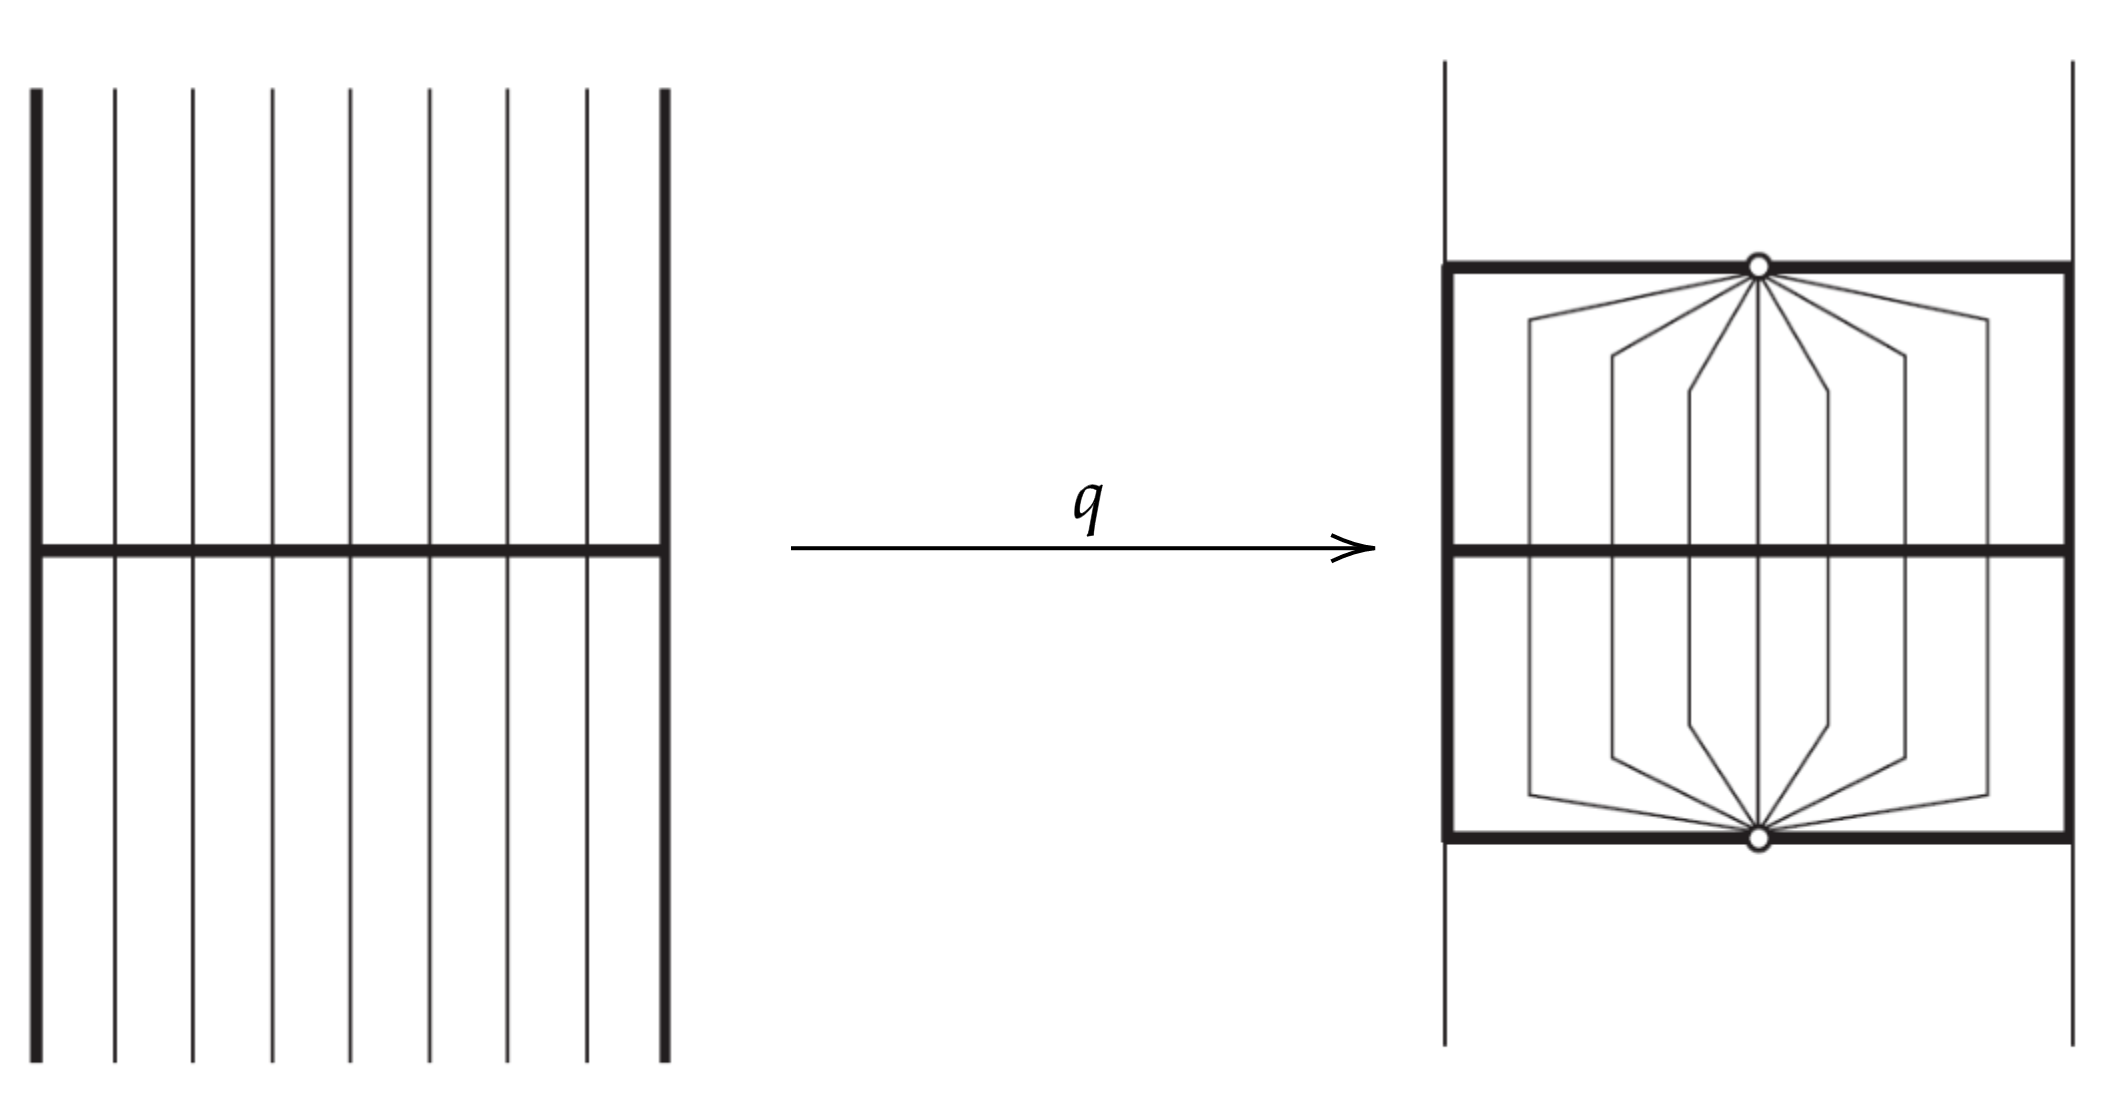
\includegraphics[width=0.5\textwidth]{embebimiento_q}
  				\label{fig:embebimiento_q}
			\end{figure}
			
			Definimos $G:  ((D^1\times D^1) - (0 \times \partial D^1))_{E_1} \rightarrow (D^1\times D^1) - (0 \times \partial D^1)$ por $G = q \circ g \circ q^{-1}$, que como es la identidad entorno al borde del dominio, se puede extender a $G:\mathbb{R}^2_{E_1} \rightarrow \mathbb{R}^2$. No hay problema en los dos puntos de $0 \times \partial D^1$ ya que por como se define $q$, en ambos tiene límite y es la identidad. Su comportamiento entorno a $D^1 \times 0$ es igual que el de $g$ ($q$ es la identidad) y es la identidad fuera de $D^1 \times D^1$ y entorno a $\partial D^1 \times \mathbb{R}$.\\
			
			\begin{figure}[h]
  				\centering
  				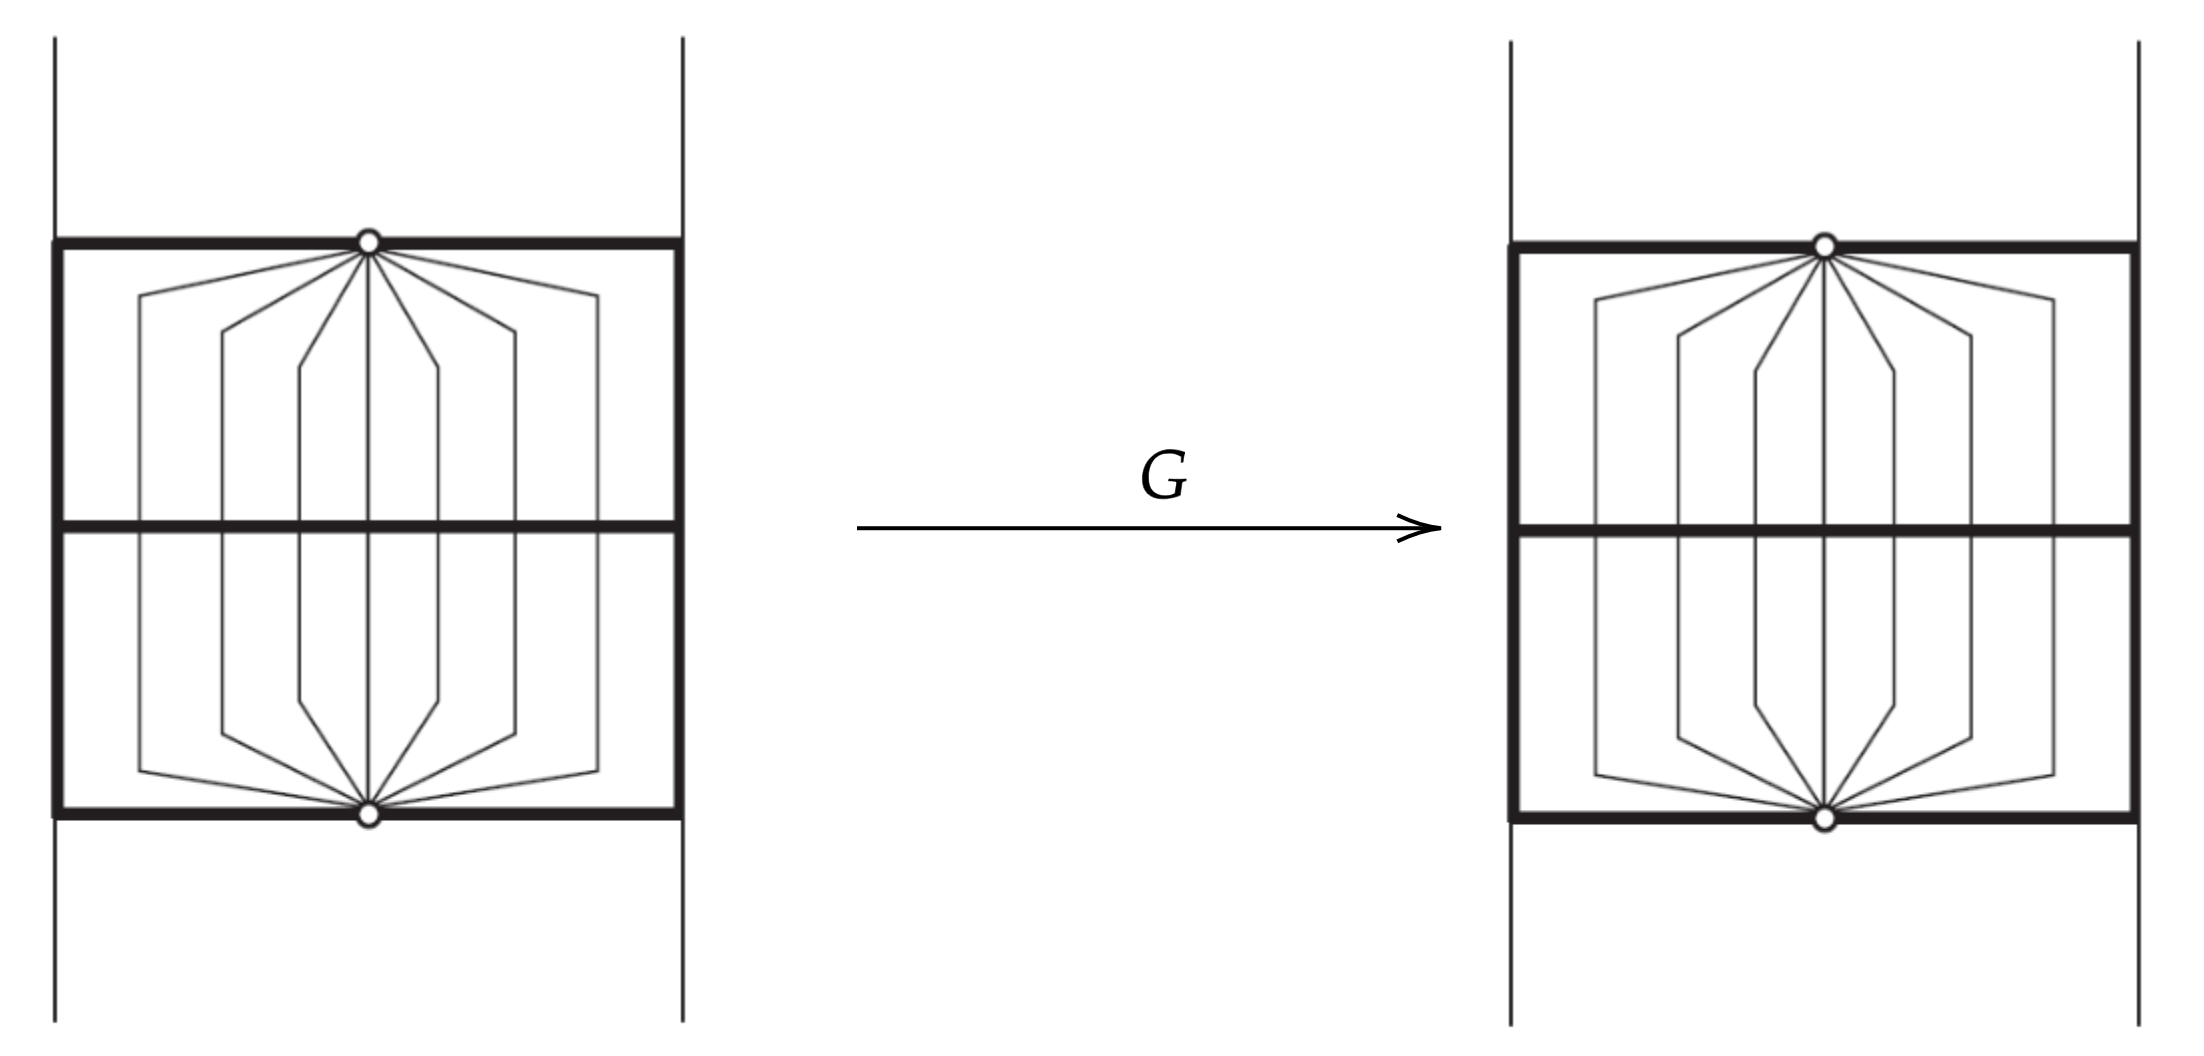
\includegraphics[width=0.5\textwidth]{g_inicial_extension}
  				\label{fig:g_inicial_extension}
			\end{figure}
			
			Podemos adaptar el truco de Alexander definiendo una isotopía $G_t$ de homemomorfismos en $\mathbb{R}^2$ rescalando el cuadrado $D^1 \times D^1$ al igual que en el apartado anterior hicimos con el disco, de forma que $G$ sea isotópica a la identidad en $\mathbb{R}^2$.\\
			\\ Finalmente basta con definir $h_t = h \circ G_t^{-1}$. Cumple claramente que $h_0 = h$, $h_1$ es diferenciable en un entorno de $D^1 \times 0$ y $h_t$ es la identidad en un entorno de $\partial D^1 \times \mathbb{R}$.
		\item Tenemos $h: D^2 \rightarrow S$ embebimiento que es diferenciable entorno al borde del dominio. Este embebimiento induce mediante ``pull-back'' la estructura diferenciable de $S$ a $D^2$ que coincide con la estructura diferenciable estándar de $D^2$ en un entorno del borde, ya que $h$ es diferenciable en dicha zona en el sentido usual.\\
			\\ Por el $\textbf{Hecho 6}$ existe un difeomorfismo $g$ entre $D^2$ con la estructura estándar y la inducida, que además es la identidad entorno al borde. Una adaptación del truco de Alexander al disco nos aporta la isotopía $g_t$ de homeomorfismos de $D^2$, donde $t$ va variando el tamaño de los discos de dominio e imagen de $g$ y extendiendo por la identidad, por lo que $g_0$ sería la identidad y $g_1 = g$. Tomando la isotopía $h_t = h \circ g_t$ tendríamos lo solicitado, ya que $h_0 = h$ y $h_1$ es igual que $h$ en un entorno del borde y es diferenciable en todo el disco.
	\end{enumerate}
	
\end{proof}


\begin{corolario}
	El primer apartado del teorema anterior sigue siendo cierto para un abierto $W$ de $\mathbb{R}^2$ en vez de para todo $\mathbb{R}^2$, con el objetivo de suavizarlo en un punto $p \in W$.
\end{corolario}

\begin{proof}
	Se restringe $h$ a $B_p \subset W$, una bola cerrada con centro $p$. Sabemos que existe $f: D^2 \rightarrow B_p$ difeomorfismo y $g=h \circ f$ se puede extender continuamente a $\mathbb{R}^2$ (al punto $q$ fuera de $D^2$ se le asigna el mismo valor que al punto de intersección de la circunferencia con el segmento del origen a $q$). Aplicamos el teorema anterior a $g:\mathbb{R}^2 \rightarrow S$ de manera que el entorno del origen $V$ donde se altera $g$ sea menor que la bola cerrada unidad, obteniendo así una isotopía $g_t$.\\
	\\Definimos la isotopía deseada como $h_t(x) = (g_t|_{D^2} \circ f^{-1})(x)$ si $x \in B_p$ y $h_t(x) = h(x)$ si $x \not \in B_p$. Está bien definida puesto que $g_t|_{D^2} \circ f^{-1}$ es la identidad fuera de un entorno de $p$ contenido en $B_p$ y simplemente extendemos por la identidad. Además, de forma natural $h_0 = h$ por ser $g_0 = g$ y $h_1$ es diferenciable en un entorno de $p$ contenido en $B_p$ por serlo $g_1$ en un entorno del origen.
\end{proof}



\endinput
%------------------------------------------------------------------------------------
% FIN DEL CAPÍTULO. 
%------------------------------------------------------------------------------------
